\documentclass[tikz, preview=true, border=2mm]{standalone}

\renewcommand*\familydefault{\sfdefault}

\usepackage{tikz}
\usetikzlibrary{mindmap,trees,shadows}

\begin{document}

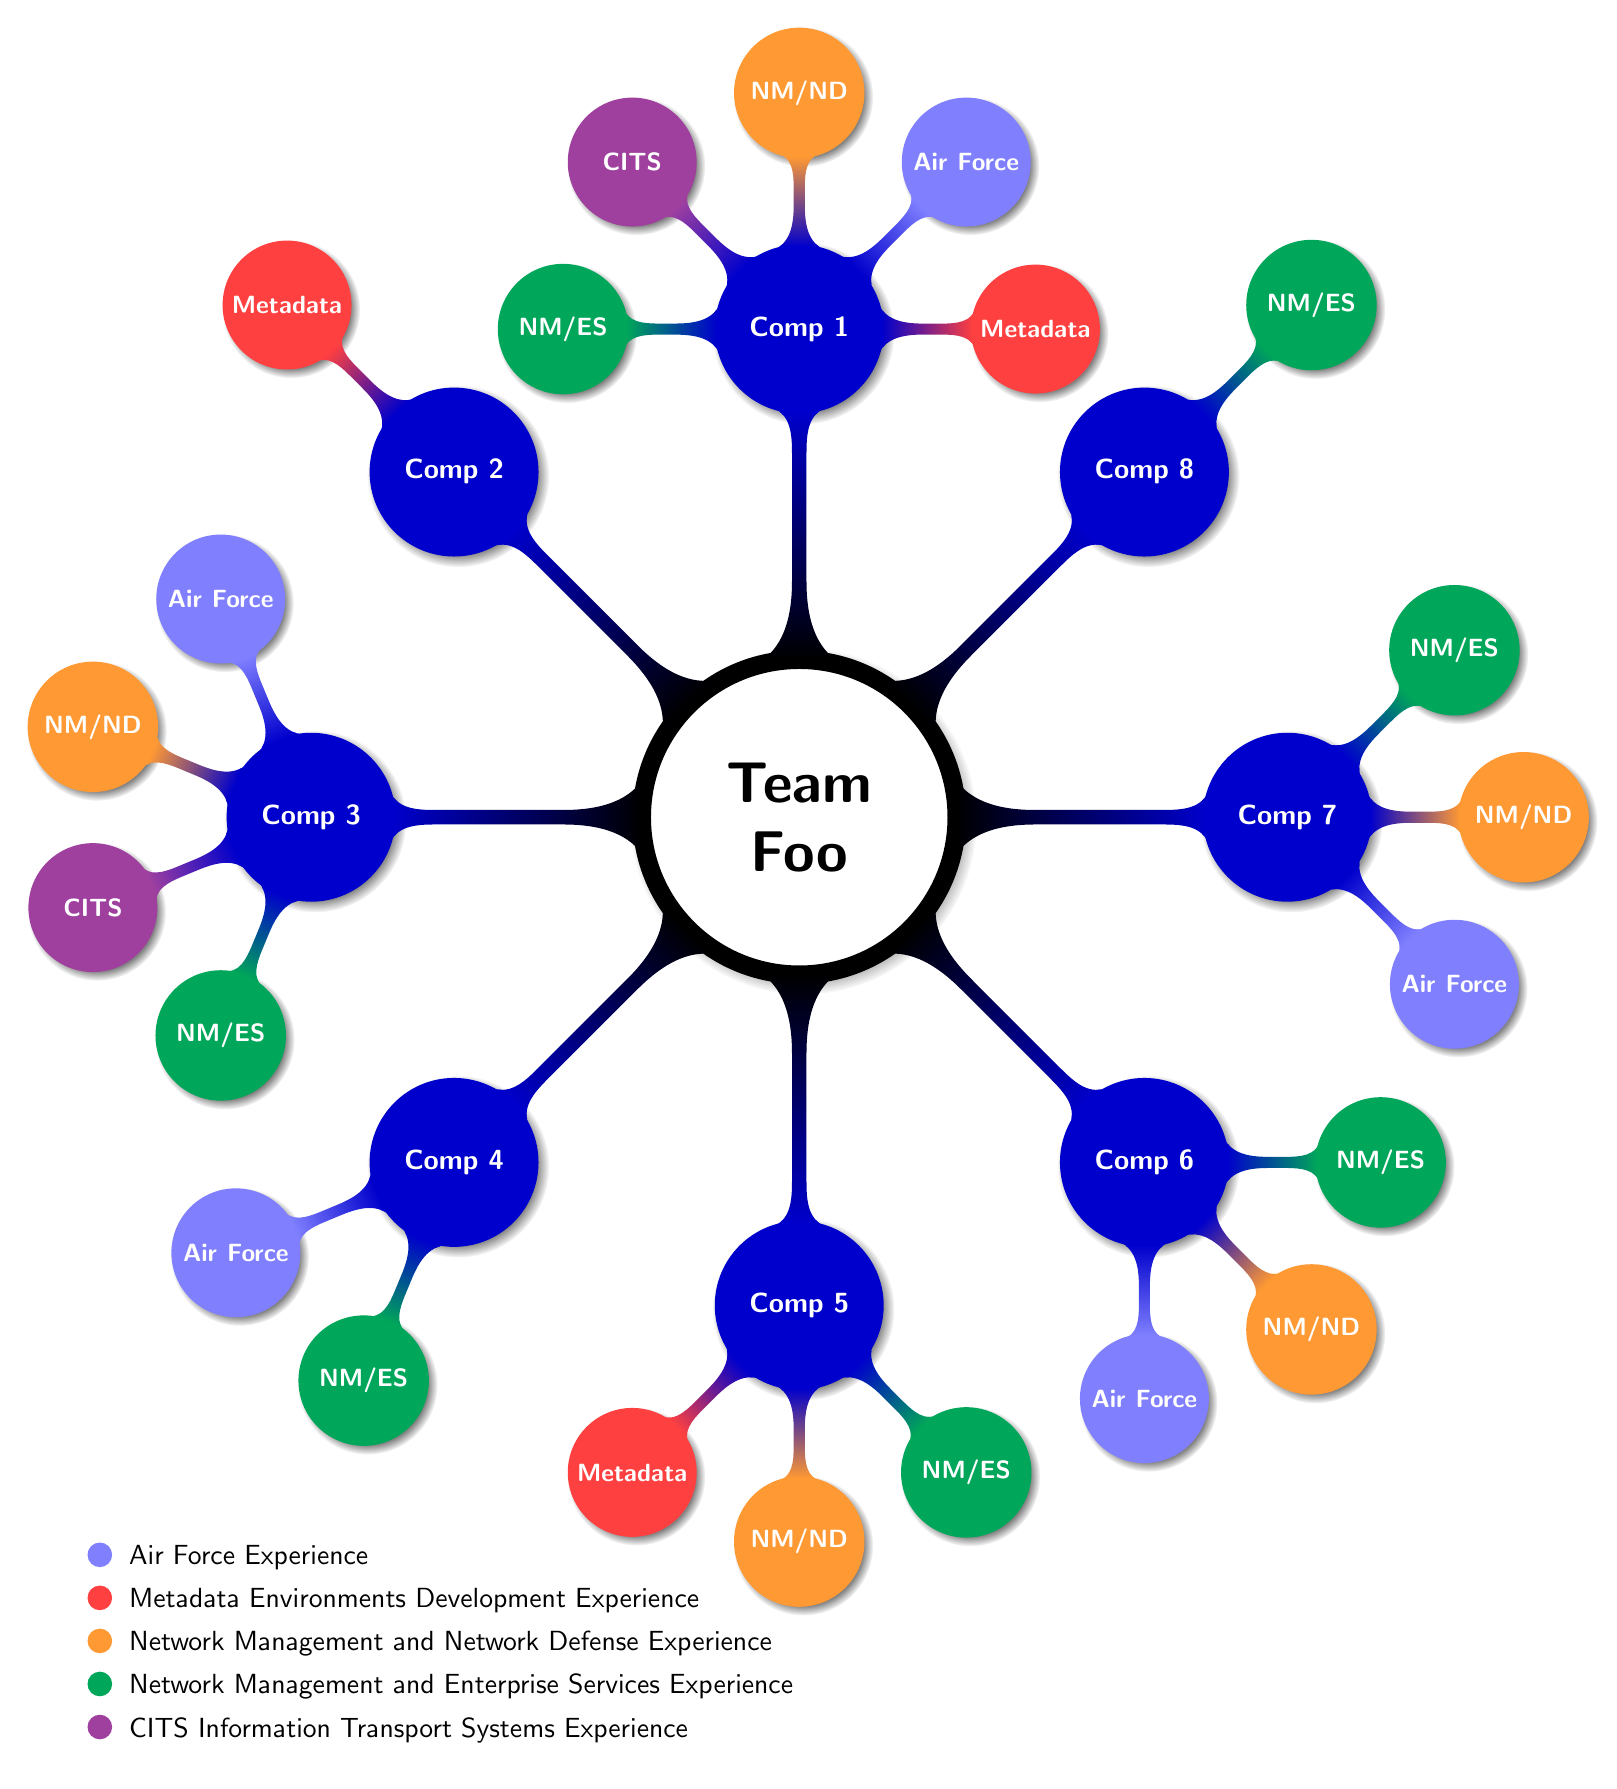
\begin{tikzpicture}
[decoration={start radius=1cm, end radius=.5cm,amplitude=3mm,angle=30}]

% Define experience colors
\colorlet{afcolor}{blue!50}
\colorlet{mdcolor}{red!75}
\colorlet{nmndcolor}{orange!80}
\colorlet{nmescolor}{teal!70!green}
\colorlet{citscolor}{violet!75}

\begin{scope}[mindmap,
every node/.style={concept, circular drop shadow, minimum size=0pt,execute at begin node=\hskip0pt, font=\bfseries},
root concept/.append style={
    concept color=black, fill=white, line width=1.5ex, text=black, font=\huge\scshape\bfseries,},
level 1 concept/.append style={font=\bfseries},
text=white,
partner/.style={concept color=blue!80!black},
air force/.style={concept color=afcolor},
metadata/.style={concept color=mdcolor},
nmnd/.style={concept color=nmndcolor},
nmes/.style={concept color=nmescolor},
cits/.style={concept color=citscolor},
grow cyclic,
level 1/.append style={level distance=6.2cm,sibling angle=45},
level 2/.append style={level distance=3cm,sibling angle=45}]
\node [root concept] (team) {Team\\Foo}[rotate=202.5] % root
    child [partner] { node {Comp 8}
        child [nmes] { node {\small NM/ES} }
    }
    child [partner] { node {Comp 1}
        child [metadata] { node {\small Metadata} }
        child [air force] { node {\small Air Force} }
        child [nmnd] { node {\small NM/ND} }
        child [cits] { node {\small CITS} }
        child [nmes] { node {\small NM/ES} }
    }
    child [partner] { node {Comp 2}
        child [metadata] { node {\small Metadata} }
    }
    child [partner] { node (comp3) {Comp 3}
        child [air force] { node {\small Air Force} }
        child [nmnd] { node {\small NM/ND} }
        child [cits] { node (leftmost) {\small CITS} }
        child [nmes] { node {\small NM/ES} }
    }
    child [partner] { node {Comp 4}
        child [air force] { node {\small Air Force} }
        child [nmes] { node {\small NM/ES} }
    }
    child [partner] { node {Comp 5}
        child [metadata] { node {\small Metadata} }
        child [nmnd] { node {\small NM/ND} }
        child [nmes] { node {\small NM/ES} }
    }
    child [partner] { node {Comp 6}
        child [air force] { node {\small Air Force} }
        child [nmnd] { node {\small NM/ND} }
        child [nmes] { node {\small NM/ES} }
    }
    child [partner] { node {Comp 7}
        child [air force] { node {\small Air Force} }
        child [nmnd] { node {\small NM/ND} }
        child [nmes] { node {\small NM/ES} }
    };
\end{scope}

\begin{scope}[xshift=-4.5cm, yshift=-10.5cm,every node/.style={align=left,text=black}]
\matrix[row sep=0pt,column sep=1mm, align=left, nodes={align=left, anchor=west}] {
    \fill [afcolor] (0,.25ex) circle (1ex); & \node{Air Force Experience};\\
    \fill [mdcolor] (0,.25ex) circle (1ex); & \node{Metadata Environments Development Experience};\\
    \fill [nmndcolor] (0,.25ex) circle (1ex); & \node{Network Management and Network Defense Experience};\\
    \fill [nmescolor] (0,.25ex) circle (1ex); & \node{Network Management and Enterprise Services Experience};\\
    \fill [citscolor] (0,.25ex) circle (1ex); & \node{CITS Information Transport Systems Experience};\\
    };
\end{scope}
\end{tikzpicture}

\end{document}